\section{Melanoma Diagnosis and Screening}\label{sec:chp1sec4}
The clinical prognosis of early stage melanoma is commonly done via visual inspection of the lesions, based on a set of rules or guidelines, such as ``ABCDE''~\cite{abbasi2004early} or Glasgow 7-point checklist~\cite{abbasi2004early}.
The ``ABCDE'' rule characterizes the lesion based on its asymmetry (A), irregular borders (B), variegated colors (C), diameter $\geq$ 6  \si{\milli\meter} (D) and evolving stage over time (E).
The Glasgow 7-point checklist contains 7 criteria: 3 major (changes in size, shape and color) and 4 minor (diameter $\geq$ 7\si{\milli\meter}, inflammation, crusting or bleeding, and sensory change). 
The former rule has been extensively used in clinical routine, rather than the latter one, due to its simplicity.


The visual inspection of lesions is carried out using different non-invasive imaging techniques such as: clinical photography, dermoscopy, \acf{clsm}, \acf{oct}, \acf{msi}, high frequency \acf{us1}, and \acf{mri} among other spectroscopic imaging. 
Concerning the aforementioned techniques, some are well-utilized by clinicians and dermatologists. 
We will refer here and after to these techniques as ``conventional'' techniques.
Clinical photography, dermoscopy, \ac{oct}, and \ac{clsm} belong to this category. 
While the rest, such as \ac{mri}, \ac{us1}, \ac{msi} and \ac{pi} are categorized as ``non-conventional'' techniques.  

We focus our research on conventional techniques such as clinical and dermoscopy as well as non-conventional techniques such as \ac{pi}. 

\subsection{Clinical photography}
Clinical photographs are referred to as digital or non-digital images captured from the surface of the skin, showing one or more lesions. 
These images reproduce what a clinician sees with the naked eye~\cite{day2000automated} and are commonly tainted with unnecessary highlights and reflections from the outer layer of the epidermis. 
The left column of Fig.\,\ref{fig:fig2} shows such images. 
%Breslow thickness 0.8 \si{\milli\meter},
\begin{figure}\centering
\subfloat[In situ melanoma (stage 0)]{
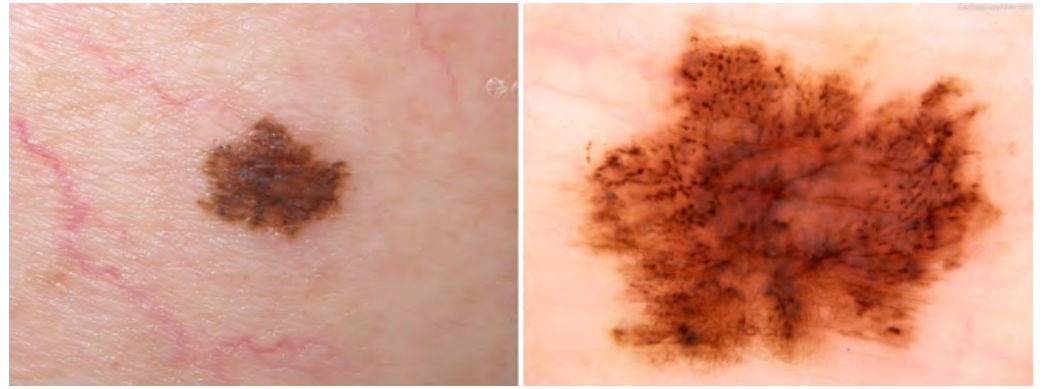
\includegraphics[width = 0.5\textwidth]{Chapter1/Figuers/CD1.png}	}\\
\subfloat[Invasive melanoma ( stage I/II)]{
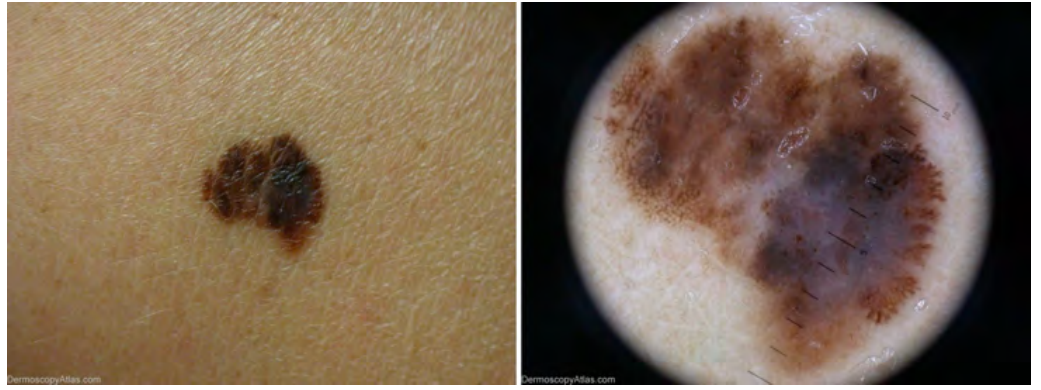
\includegraphics[width = 0.5\textwidth]{Chapter1/Figuers/CD2.png}	}
	\caption[Clinical and dermoscopy images]{Clinical and Dermoscopy images, right and left column, respectively. Images submitted
to www.dermoscopyatlas.com by Dr. Alan Cameron (a), Dr. Jean-Yves Gourhant (b). Used with permission.}
\label{fig:fig2}
\end{figure}

\subsection{Dermoscopy}
\label{subsec:derm}
Dermoscopy (also known as dermatoscopy or epiluminescence microscopy) is a well-established and effective non-invasive technique for early recognition of melanoma. 
This technique, introduced in 1971~\cite{mackie1972cutaneous, mackie1971aid}, uses a hand-held lighted magnifier to analyze skin lesions. 

Initially the device was used in conjunction with a thin layer of glass and an oil or alcohol interface to reduce light reflection, refraction and diffraction.
This material made the epidermis translucent and allowed in vivo visualization of subsurface anatomic structures of the epidermis and papillary dermis which are not visible with naked eye~\cite{rigel2010evolution,wang2010noninvasive}.
This first type of dermoscopes is called a \ac{npd}~\cite{wang2010noninvasive}. 

The second type, the \acf{pd}, was introduced later and made this process much easier by using cross-polarized light. 
This device is equipped with two polarized filters, one in front of the light source and one in front of the sensor. 
The two polarized filters are perpendicular to each other in order to capture the backscattered light from the deeper levels of the skin. 
The light reflected from the skin has the same angle as the polarized incident light, hence it is eliminated with the cross-polarized filter in front of the sensor. 
However, the backscattered light from the skin, due to the structural nature of the tissue, will become unpolarized and passes through the filter.
This technique eliminates the need for fluid or direct contact with the skin.

A sample of commercially available dermoscopes (Dermlite$^{\circledR}$) with and without polarized light are shown in Fig~\ref{fig:fig4}.
MoleMax (Derma Medical System, Vienna, Austria) is another commercially available system that includes a polarized dermoscope.
MoleMax is a computer based device and by providing its own software, allows live-video dermoscopy and total body photography~\cite{marghoob2003instruments,rigel2010evolution}.

\begin{figure}[h]
\centering
\subfloat[Dermlite$^{\circledR}$ II Fluid]{
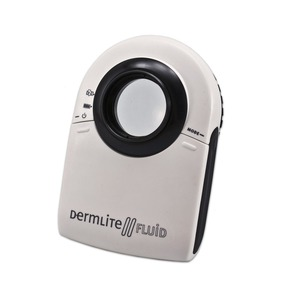
\includegraphics[width = 0.3\textwidth]{Chapter1/Figuers/Dermlite_fluid.jpg}	}
\subfloat[Dermlite$^{\circledR}$ II Pro HR]{
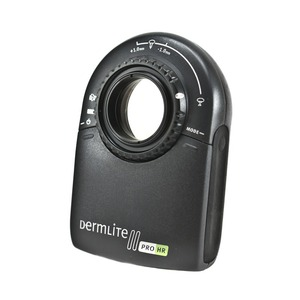
\includegraphics[width = 0.3\textwidth]{Chapter1/Figuers/Dermlite_PD.jpg}	}
\caption[Dermoscopes]{Commercially available dermoscopes by Dermlite$^{\circledR}$:  (a) immersion fluid dermoscope using non-polarized light; (b) cross-polarized light dermoscope. Both devices can be attached to a digital camera.}
\label{fig:fig4}
\end{figure}

The images captured using a \ac{pd} or a \ac{npd} are relatively similar.
However, the surface dermoscopic structures (such as the blue white veil) are better observed with a \ac{npd} while deep structures (such as vessels) are better seen with a \ac{pd}~\cite{wang2010noninvasive, benvenuto2007differences}.
The right column of Fig~\ref{fig:fig2} demonstrates the dermoscopic images of the same lesions captured with an \ac{npd}.
Figure~\ref{fig:fig3} shows difference of clinical, \ac{npd}, and \ac{pd} imaging for a melanoma lesion.

\begin{figure}\centering
\subfloat[Clinical]{
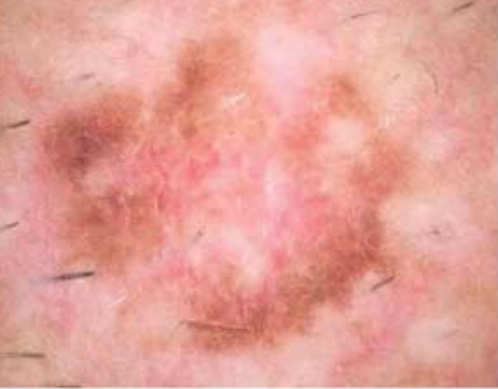
\includegraphics[width = 0.33\textwidth]{Chapter1/Figuers/Melanoma_Clinical.png}}
\subfloat[\ac{npd} ]{
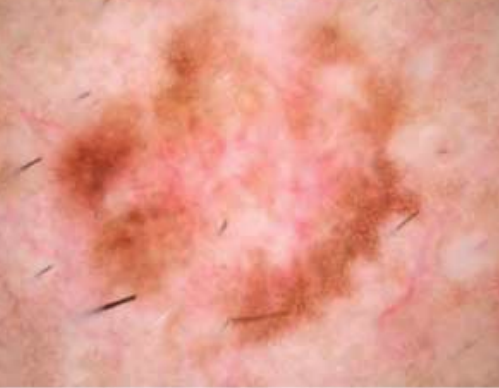
\includegraphics[width = 0.33\textwidth]{Chapter1/Figuers/Melanoma_NPD.png}}
\subfloat[\ac{pd} ]{
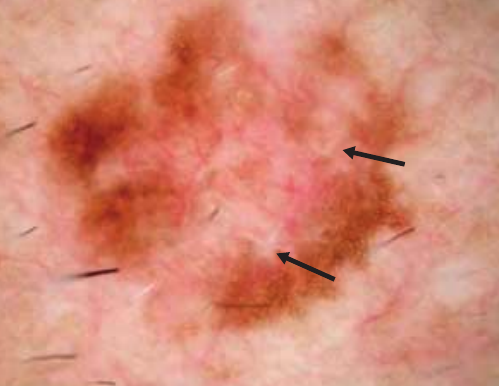
\includegraphics[width = 0.33\textwidth]{Chapter1/Figuers/Melanoma_PD.png}}
	\caption[Clinical, \ac{npd} and \ac{pd} images of melanoma]{Melanoma lesion captured by clinical photography,  An \ac{npd}, and a \ac{pd}, respectively. Shiny white streaks (arrow in (c)) within the melanoma are only visible with the \ac{npd}. The images are taken from Benvenuto~et al.~\cite{benvenuto2007differences}}
\label{fig:fig3}
\end{figure}


Besides the \ac{npd} and the \ac{pd}, another dermoscopy technique, via transillumination, was introduced by Dhawan~et.al.~\cite{Dhawan1985,Dhawan1984}.
In this technique, light is directed to the skin in such a way that allows the backscattered light to illuminate the lesion from within. 
Novescope is a patented device developed for this technique. 
%Figure~\ref{fig:fig5} shows a schematic of this design. The device used for this design is patented and called Nevoscope~\cite{Dhawan1985,Dhawan1984}. 
 


%%% Ask for permission first. 
%\begin{figure}[h]
%\centering
%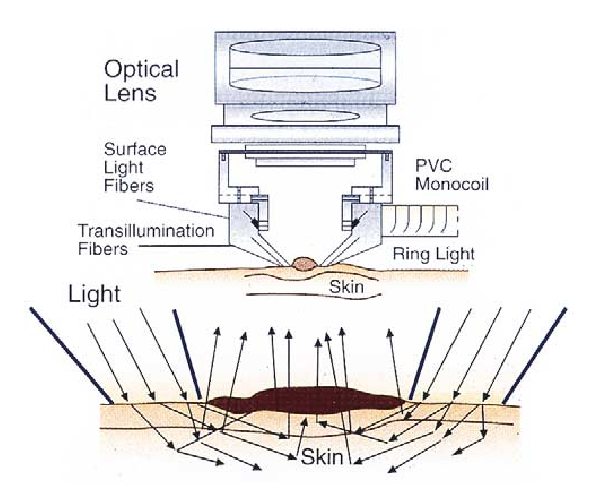
\includegraphics[width = 0.3\textwidth]{Chapter1/Figures/Nevoscope.jpg}	
%\caption{Dermoscopy techniques by transillumination oflesion (Nevoscope)}
%\label{fig:fig5}
%\end{figure}

% for more information the interested reader can refer to : Marghoob 2003, Quintana 2012, L.Smith 2011, Rigel 2010, Wang 2010, Gadeliya 2009, Pstay 2009, Esmaili 2008, Patel 2008  
%\subsection{Confocal Laser Scanning Microscopy}
%\ac*{clsm} is another non-invasive technique, that provides real time in-vivo images of skin at variable depths in horizontal planes equivalent to the resolution of conventional microscope~\cite{rigel2010evolution}. 
%The high resolution of the microscope allows to capture nuclear, cellular, and tissue architectures of the epidermis and underlying structures, without any biopsy.
%In comparison to fluorescence microscopic , the skin is difficult to investigate because it reflects and scatters incoming light and melanin and other chromophores, significantly attenuate visible wavelength. 
%\subsection{Optical Coherence tomography}

\subsection{Polarized imaging}
In \acf{pi} or image polarimetry systems a polarizer state generator and analyzer are used to create a set of polarized images. 
These images define the polarization state of the light beam and the depolarization property of the tissue.
The former is represented by four measurable quantities called Stokes parameters and the later is represented by the Mueller matrix. 
The advantage and benefits of \ac{pi} systems besides being cross-polarized are not as evident in the field of skin imaging or tissue imaging in general.
Over the last few decades, few studies have been dedicated to finding and exploring the depolarization properties of tissues~\cite{Anastasiadou2008,manhas2009polarized,manhas2009polarized,Jacques12175282}
%Anastasiadou~et al.\ proposed a Mueller polarimetry system for diagnosing the cervical cancer \cite{Anastasiadou2008} and Manhas~et al.\ proposed a Mueller polarimetry system for measuring polarized diffuse reflectance on cancerous and non-cancerous regions of oral cavity and breast tissues \cite{manhas2009polarized}. 
%In the field of skin tissue, Jacques~et al.\ proposed Stokes polarimetry to differentiate different pigmented lesions \cite{}. 
%Another work recently was proposed by Tchvialeva~et al.\ where polarized speckle imaging was suggested for in vivo screening of pigmented lesions \cite{manhas2009polarized}. 
The Stokes and Mueller measurements along with the basics of polarization and the methods proposed by the research community are further explained in Chap.\,\ref{chp:chapter4}
%The Stokes polarimetry, Mueller matrix measurements, and the proposed methods by the research community are further explained in Chapt.\,\ref{chp:chapter4}.


%\subsection{Multispectral Imaging}
%In multispectral imaging, a set of wavelength dependent images are acquired in order to visualize different depths and layers of the skin. 
%This is possible since depth of light penetration into the skin is directly related to wavelength. 
%The wavelengths can range from \ac{uv} to \ac{nir}. 
%This technique offers the advantage of analyzing the sub-layers which are not visible to the human eye, probing up to 2 \si{\milli\meter} below the surface of the skin~\cite{rigel2010evolution}~(see Fig.~\ref{fig:MSI_ex1}).

%\begin{figure}[h]\centering
%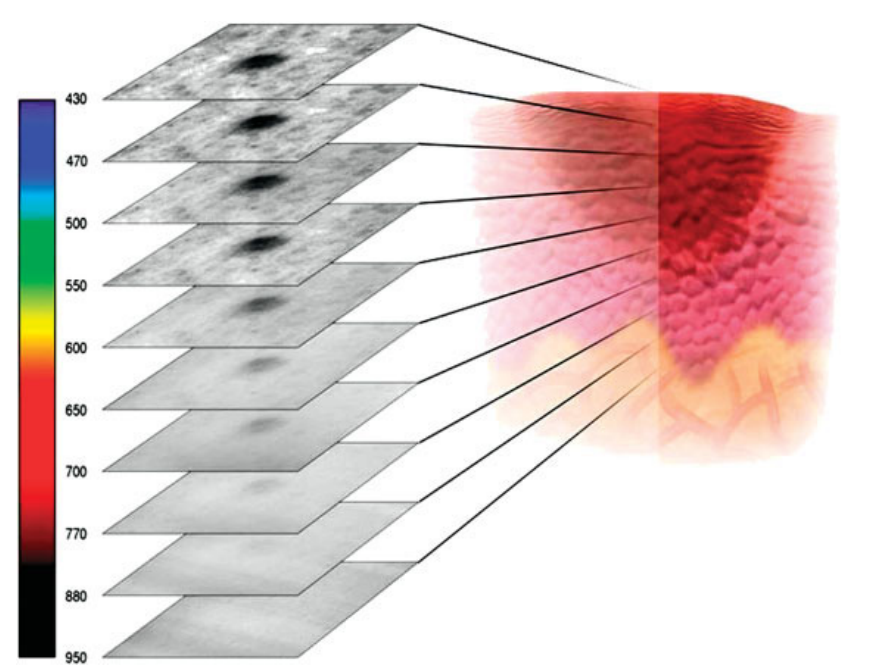
\includegraphics[scale=0.5]{Chapter1/Figuers/MS_example.png}
%\caption[Multispectral analysis of pigmented skin lesions]{Multispectral analysis of pigmented skin lesion. Longer wavelength penetrates deeper into the skin, providing diagnostic features. The image is taken from Rigel~et al.~\cite{rigel2010evolution} }
%\label{fig:MSI_ex1}
%\end{figure} 
%Opposed to standard color cameras which capture the skin image in three channels (red, green, blue), \ac{msi} acquires a sequence of gray level images at different wavelengths. 
%This extended spectral capacity provides a high advantage in skin imaging since it is reducing the effects of metameric mismatches, which may occur due to different illumination and variability of sensor spectral responses \cite{jolivot2011developpement}.
%The spectral device of \ac{msi} can be placed either along the incident path, or in detection path.
%In either way, the main motivation is to go beyond the limited red, green and blue color information which are available by other imaging techniques. 
%This technique combines the advantage of both a spectrophotometer and a digital camera. 
%The \ac{msi} system acquires three-dimensional data, the spatial information in 2 dimensions and a spectral information in the third dimension, obtaining spectral information for each pixel in the image. 	
%	
%Currently, several multispectral dermoscopes are commercially available: MelaFind~\cite{elbaum2001automatic,Gutkowicz-Krusin1997}, SolarScan~\cite{menzies2001short,menzies2005performance}, and SIAscope~\cite{moncrieff2002spectrophotometric}. 
%This topic is extensively discussed in Chapt.\,\ref{chp:chapter5}.





  %%% Local Variables: 
  %%% mode: latex
  %%% TeX-master: "../thesis"
  %%% End